\title{WWW Analysis Note}
\author{WWW Analysis Team}
\date{\today}

\documentclass[12pt]{article}

%\usepackage[landscape]{geometry}
\usepackage{fullpage}
\usepackage{graphicx}
\usepackage{subfig}
\usepackage{verbatim}
\usepackage{xcolor}

\newcommand{\analysispath}{/home/users/phchang/public_html/analysis/www/code/WWWAnalysisRun2/analysis/plots/WWW2017_v4.0.6/test22}

\begin{document}
\maketitle

\begin{abstract}
This contains various tables and plots used for the actual AN of WWW analysis.
\end{abstract}

\section{Lost Lepton Control Region}

\input{\analysispath/lostlep_cr_yield}

\begin{figure}[htb]
    \centering
    \subfloat[][]{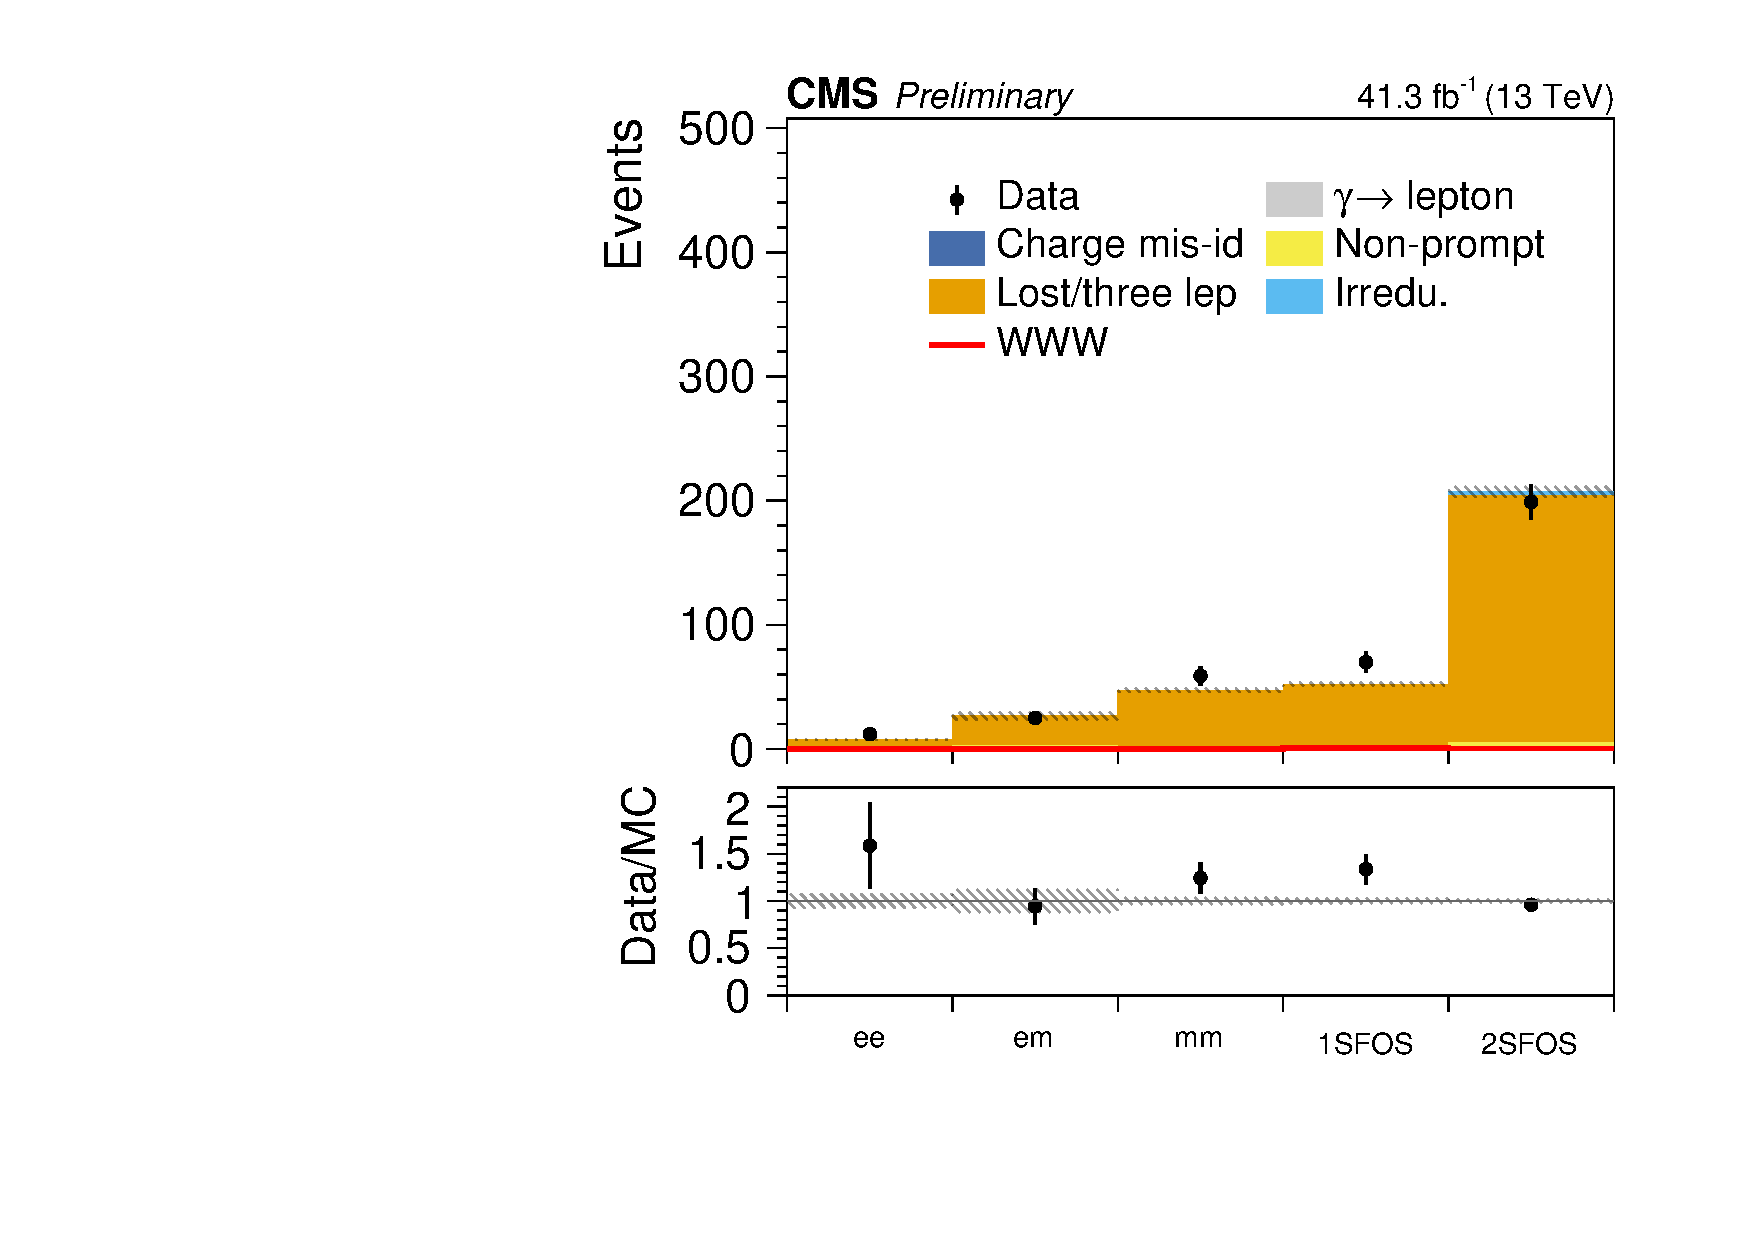
\includegraphics[width=0.45\textwidth]{\analysispath/lostlep_cr_yield.pdf}}
    \caption{
        \label{fig:2017:lostlepcr} Lost lepton control region for 2017 data.
    }
\end{figure}


\input{\analysispath/lostlep_exp_syst}

\begin{figure}[htb]
    \centering
    \subfloat[][]{\includegraphics[width=0.45\textwidth]{\analysispath/lostlep_cr_ss_msfos.pdf}\label{fig:2017:lostlepcr:msfos:ss}}
    \subfloat[][]{\includegraphics[width=0.45\textwidth]{\analysispath/lostlep_cr_3l_msfos.pdf}\label{fig:2017:lostlepcr:msfos:3l}}\\
    \subfloat[][]{\includegraphics[width=0.45\textwidth]{\analysispath/lostlep_cr_ss_mjj.pdf}\label{fig:2017:lostlepcr:mjj:ss}}
    \caption{
        \label{fig:2017:lostlepcr:modeling} Lost lepton control region, efficiencies and extrapolation checks
        \subref{fig:2017:lostlepcr:msfos:ss}{ The $m_{SFOS}$ distribution in lost lepton control regions for same-sign channels.} 
        \subref{fig:2017:lostlepcr:msfos:3l}{ The $m_{SFOS}$ distribution in lost lepton control regions for three-lepton channels.} 
        \subref{fig:2017:lostlepcr:mjj:ss}{ The $m_{jj}$ distribution in lost lepton control regions for same-sign channels.} 
    }
\end{figure}

\input{\analysispath/lostlep_eff_msfos_ss}
\input{\analysispath/lostlep_ratio_msfos_3l}
\input{\analysispath/lostlep_eff_mjj_ss}

\clearpage

\section{Statistical interpretation}

\subsection{$m_{jj}$-in ee}
\scalebox{0.4}{\parbox{2.0\textwidth}{\verbatiminput{/home/users/phchang/public_html/analysis/www/code/WWWAnalysisRun2/analysis/plots/WWW2017_v4.0.6/test22/datacard_SRSSee.txt}}}
\subsection{$m_{jj}$-in em}
\scalebox{0.4}{\parbox{2.0\textwidth}{\verbatiminput{/home/users/phchang/public_html/analysis/www/code/WWWAnalysisRun2/analysis/plots/WWW2017_v4.0.6/test22/datacard_SRSSem.txt}}}
\subsection{$m_{jj}$-in mm}
\scalebox{0.4}{\parbox{2.0\textwidth}{\verbatiminput{/home/users/phchang/public_html/analysis/www/code/WWWAnalysisRun2/analysis/plots/WWW2017_v4.0.6/test22/datacard_SRSSmm.txt}}}
\subsection{$m_{jj}$-out ee}
\scalebox{0.4}{\parbox{2.0\textwidth}{\verbatiminput{/home/users/phchang/public_html/analysis/www/code/WWWAnalysisRun2/analysis/plots/WWW2017_v4.0.6/test22/datacard_SRSSSideee.txt}}}
\subsection{$m_{jj}$-out em}
\scalebox{0.4}{\parbox{2.0\textwidth}{\verbatiminput{/home/users/phchang/public_html/analysis/www/code/WWWAnalysisRun2/analysis/plots/WWW2017_v4.0.6/test22/datacard_SRSSSideem.txt}}}
\subsection{$m_{jj}$-out mm}
\scalebox{0.4}{\parbox{2.0\textwidth}{\verbatiminput{/home/users/phchang/public_html/analysis/www/code/WWWAnalysisRun2/analysis/plots/WWW2017_v4.0.6/test22/datacard_SRSSSidemm.txt}}}
\subsection{0SFOS}
\scalebox{0.4}{\parbox{2.0\textwidth}{\verbatiminput{/home/users/phchang/public_html/analysis/www/code/WWWAnalysisRun2/analysis/plots/WWW2017_v4.0.6/test22/datacard_SR0SFOS.txt}}}
\subsection{1SFOS}
\scalebox{0.4}{\parbox{2.0\textwidth}{\verbatiminput{/home/users/phchang/public_html/analysis/www/code/WWWAnalysisRun2/analysis/plots/WWW2017_v4.0.6/test22/datacard_SR1SFOS.txt}}}
\subsection{2SFOS}
\scalebox{0.4}{\parbox{2.0\textwidth}{\verbatiminput{\analysispath/datacard_SR2SFOS.txt}}}


\end{document}
